% Created by tikzDevice version 0.12.6 on 2024-09-14 08:06:38
% !TEX encoding = UTF-8 Unicode
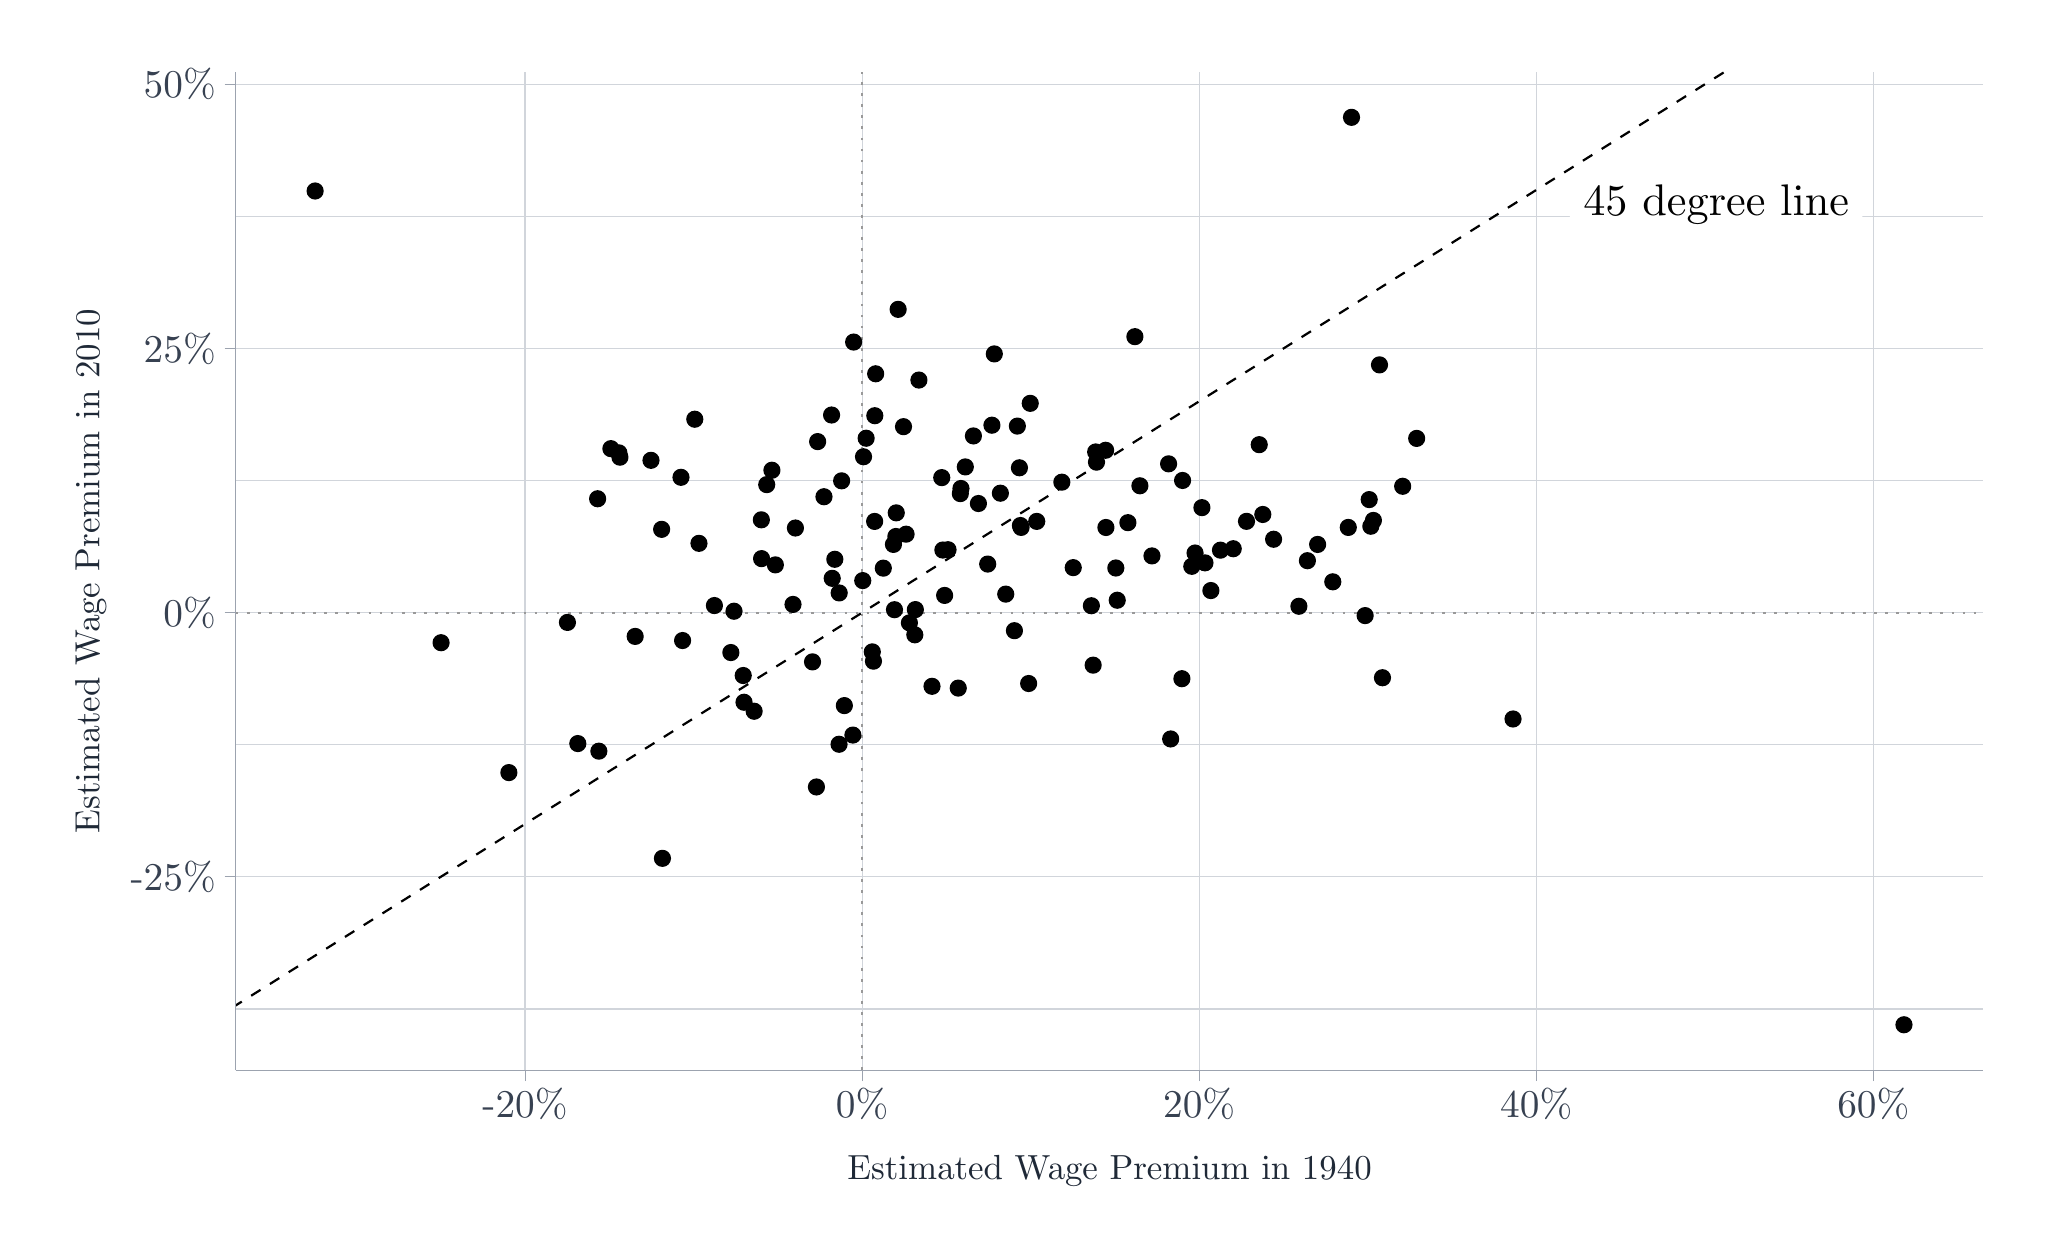
\begin{tikzpicture}[x=1pt,y=1pt]
\definecolor{fillColor}{RGB}{255,255,255}
\path[use as bounding box,fill=fillColor] (0,0) rectangle (722.70,433.62);
\begin{scope}
\path[clip] (  0.00,  0.00) rectangle (722.70,433.62);
\definecolor{drawColor}{RGB}{255,255,255}

\path[draw=drawColor,line width= 0.8pt,line join=round,line cap=round,fill=fillColor] ( -0.00,  0.00) rectangle (722.70,433.62);
\end{scope}
\begin{scope}
\path[clip] ( 75.17, 56.92) rectangle (706.70,417.62);
\definecolor{drawColor}{RGB}{255,255,255}
\definecolor{fillColor}{RGB}{255,255,255}

\path[draw=drawColor,line width= 0.8pt,line join=round,line cap=round,fill=fillColor] ( 75.17, 56.92) rectangle (706.70,417.62);
\definecolor{drawColor}{RGB}{209,213,219}

\path[draw=drawColor,line width= 0.4pt,line join=round] ( 75.17, 79.02) --
	(706.70, 79.02);

\path[draw=drawColor,line width= 0.4pt,line join=round] ( 75.17,174.49) --
	(706.70,174.49);

\path[draw=drawColor,line width= 0.4pt,line join=round] ( 75.17,269.96) --
	(706.70,269.96);

\path[draw=drawColor,line width= 0.4pt,line join=round] ( 75.17,365.42) --
	(706.70,365.42);

\path[draw=drawColor,line width= 0.4pt,line join=round] ( 75.17,126.76) --
	(706.70,126.76);

\path[draw=drawColor,line width= 0.4pt,line join=round] ( 75.17,222.22) --
	(706.70,222.22);

\path[draw=drawColor,line width= 0.4pt,line join=round] ( 75.17,317.69) --
	(706.70,317.69);

\path[draw=drawColor,line width= 0.4pt,line join=round] ( 75.17,413.15) --
	(706.70,413.15);

\path[draw=drawColor,line width= 0.4pt,line join=round] (179.71, 56.92) --
	(179.71,417.62);

\path[draw=drawColor,line width= 0.4pt,line join=round] (301.52, 56.92) --
	(301.52,417.62);

\path[draw=drawColor,line width= 0.4pt,line join=round] (423.32, 56.92) --
	(423.32,417.62);

\path[draw=drawColor,line width= 0.4pt,line join=round] (545.13, 56.92) --
	(545.13,417.62);

\path[draw=drawColor,line width= 0.4pt,line join=round] (666.94, 56.92) --
	(666.94,417.62);
\definecolor{drawColor}{gray}{0.60}

\path[draw=drawColor,line width= 0.8pt,dash pattern=on 1pt off 3pt ,line join=round] ( 75.17,222.22) -- (706.70,222.22);

\path[draw=drawColor,line width= 0.8pt,dash pattern=on 1pt off 3pt ,line join=round] (301.52, 56.92) -- (301.52,417.62);
\definecolor{drawColor}{RGB}{0,0,0}

\path[draw=drawColor,line width= 0.8pt,dash pattern=on 4pt off 4pt ,line join=round] (-556.37,-315.66) -- (1338.23,872.23);

\path[fill=fillColor] (560.20,360.82) --
	(660.08,360.82) --
	(659.96,360.82) --
	(660.43,360.84) --
	(660.88,360.94) --
	(661.32,361.10) --
	(661.72,361.33) --
	(662.08,361.63) --
	(662.39,361.98) --
	(662.64,362.37) --
	(662.82,362.80) --
	(662.93,363.25) --
	(662.97,363.71) --
	(662.97,363.71) --
	(662.97,378.59) --
	(662.97,378.59) --
	(662.93,379.05) --
	(662.82,379.50) --
	(662.64,379.93) --
	(662.39,380.32) --
	(662.08,380.67) --
	(661.72,380.97) --
	(661.32,381.20) --
	(660.88,381.36) --
	(660.43,381.46) --
	(660.08,381.48) --
	(560.20,381.48) --
	(560.55,381.46) --
	(560.09,381.47) --
	(559.63,381.42) --
	(559.18,381.29) --
	(558.76,381.09) --
	(558.38,380.83) --
	(558.04,380.50) --
	(557.76,380.13) --
	(557.54,379.72) --
	(557.40,379.28) --
	(557.32,378.82) --
	(557.31,378.59) --
	(557.31,363.71) --
	(557.32,363.95) --
	(557.32,363.48) --
	(557.40,363.02) --
	(557.54,362.58) --
	(557.76,362.17) --
	(558.04,361.80) --
	(558.38,361.47) --
	(558.76,361.21) --
	(559.18,361.01) --
	(559.63,360.88) --
	(560.09,360.82) --
	cycle;
\end{scope}
\begin{scope}
\path[clip] ( 75.17, 56.92) rectangle (706.70,417.62);
\definecolor{drawColor}{RGB}{0,0,0}

\node[text=drawColor,anchor=base west,inner sep=0pt, outer sep=0pt, scale=  1.60] at (562.13,365.64) {45 degree line};
\end{scope}
\begin{scope}
\path[clip] ( 75.17, 56.92) rectangle (706.70,417.62);
\definecolor{drawColor}{RGB}{0,0,0}
\definecolor{fillColor}{RGB}{0,0,0}

\path[draw=drawColor,line width= 0.5pt,line join=round,line cap=round,fill=fillColor] (677.99, 73.32) circle (  2.85);

\path[draw=drawColor,line width= 0.5pt,line join=round,line cap=round,fill=fillColor] (536.73,183.81) circle (  2.85);

\path[draw=drawColor,line width= 0.5pt,line join=round,line cap=round,fill=fillColor] (489.55,198.72) circle (  2.85);

\path[draw=drawColor,line width= 0.5pt,line join=round,line cap=round,fill=fillColor] (483.29,221.17) circle (  2.85);

\path[draw=drawColor,line width= 0.5pt,line join=round,line cap=round,fill=fillColor] (413.02,176.59) circle (  2.85);

\path[draw=drawColor,line width= 0.5pt,line join=round,line cap=round,fill=fillColor] (471.60,233.38) circle (  2.85);

\path[draw=drawColor,line width= 0.5pt,line join=round,line cap=round,fill=fillColor] (459.35,224.54) circle (  2.85);

\path[draw=drawColor,line width= 0.5pt,line join=round,line cap=round,fill=fillColor] (417.08,198.37) circle (  2.85);

\path[draw=drawColor,line width= 0.5pt,line join=round,line cap=round,fill=fillColor] (485.34,253.46) circle (  2.85);

\path[draw=drawColor,line width= 0.5pt,line join=round,line cap=round,fill=fillColor] (486.28,255.56) circle (  2.85);

\path[draw=drawColor,line width= 0.5pt,line join=round,line cap=round,fill=fillColor] (462.43,241.01) circle (  2.85);

\path[draw=drawColor,line width= 0.5pt,line join=round,line cap=round,fill=fillColor] (496.85,267.90) circle (  2.85);

\path[draw=drawColor,line width= 0.5pt,line join=round,line cap=round,fill=fillColor] (477.20,253.03) circle (  2.85);

\path[draw=drawColor,line width= 0.5pt,line join=round,line cap=round,fill=fillColor] (466.12,246.88) circle (  2.85);

\path[draw=drawColor,line width= 0.5pt,line join=round,line cap=round,fill=fillColor] (484.76,263.09) circle (  2.85);

\path[draw=drawColor,line width= 0.5pt,line join=round,line cap=round,fill=fillColor] (501.91,285.20) circle (  2.85);

\path[draw=drawColor,line width= 0.5pt,line join=round,line cap=round,fill=fillColor] (427.55,230.22) circle (  2.85);

\path[draw=drawColor,line width= 0.5pt,line join=round,line cap=round,fill=fillColor] (450.21,248.76) circle (  2.85);

\path[draw=drawColor,line width= 0.5pt,line join=round,line cap=round,fill=fillColor] (385.01,203.26) circle (  2.85);

\path[draw=drawColor,line width= 0.5pt,line join=round,line cap=round,fill=fillColor] (435.63,245.33) circle (  2.85);

\path[draw=drawColor,line width= 0.5pt,line join=round,line cap=round,fill=fillColor] (425.41,240.23) circle (  2.85);

\path[draw=drawColor,line width= 0.5pt,line join=round,line cap=round,fill=fillColor] (431.02,244.81) circle (  2.85);

\path[draw=drawColor,line width= 0.5pt,line join=round,line cap=round,fill=fillColor] (420.65,238.98) circle (  2.85);

\path[draw=drawColor,line width= 0.5pt,line join=round,line cap=round,fill=fillColor] (446.31,257.71) circle (  2.85);

\path[draw=drawColor,line width= 0.5pt,line join=round,line cap=round,fill=fillColor] (361.70,196.63) circle (  2.85);

\path[draw=drawColor,line width= 0.5pt,line join=round,line cap=round,fill=fillColor] (440.42,255.23) circle (  2.85);

\path[draw=drawColor,line width= 0.5pt,line join=round,line cap=round,fill=fillColor] (421.83,243.78) circle (  2.85);

\path[draw=drawColor,line width= 0.5pt,line join=round,line cap=round,fill=fillColor] (393.71,226.72) circle (  2.85);

\path[draw=drawColor,line width= 0.5pt,line join=round,line cap=round,fill=fillColor] (384.36,224.74) circle (  2.85);

\path[draw=drawColor,line width= 0.5pt,line join=round,line cap=round,fill=fillColor] (406.26,242.74) circle (  2.85);

\path[draw=drawColor,line width= 0.5pt,line join=round,line cap=round,fill=fillColor] (336.26,194.97) circle (  2.85);

\path[draw=drawColor,line width= 0.5pt,line join=round,line cap=round,fill=fillColor] (285.01,159.25) circle (  2.85);

\path[draw=drawColor,line width= 0.5pt,line join=round,line cap=round,fill=fillColor] (393.20,238.37) circle (  2.85);

\path[draw=drawColor,line width= 0.5pt,line join=round,line cap=round,fill=fillColor] (424.31,260.18) circle (  2.85);

\path[draw=drawColor,line width= 0.5pt,line join=round,line cap=round,fill=fillColor] (356.56,215.72) circle (  2.85);

\path[draw=drawColor,line width= 0.5pt,line join=round,line cap=round,fill=fillColor] (326.78,195.62) circle (  2.85);

\path[draw=drawColor,line width= 0.5pt,line join=round,line cap=round,fill=fillColor] (298.19,178.00) circle (  2.85);

\path[draw=drawColor,line width= 0.5pt,line join=round,line cap=round,fill=fillColor] (293.19,174.68) circle (  2.85);

\path[draw=drawColor,line width= 0.5pt,line join=round,line cap=round,fill=fillColor] (229.37,133.46) circle (  2.85);

\path[draw=drawColor,line width= 0.5pt,line join=round,line cap=round,fill=fillColor] (488.48,311.77) circle (  2.85);

\path[draw=drawColor,line width= 0.5pt,line join=round,line cap=round,fill=fillColor] (445.02,282.93) circle (  2.85);

\path[draw=drawColor,line width= 0.5pt,line join=round,line cap=round,fill=fillColor] (377.81,238.50) circle (  2.85);

\path[draw=drawColor,line width= 0.5pt,line join=round,line cap=round,fill=fillColor] (397.56,254.75) circle (  2.85);

\path[draw=drawColor,line width= 0.5pt,line join=round,line cap=round,fill=fillColor] (417.32,270.00) circle (  2.85);

\path[draw=drawColor,line width= 0.5pt,line join=round,line cap=round,fill=fillColor] (295.10,188.65) circle (  2.85);

\path[draw=drawColor,line width= 0.5pt,line join=round,line cap=round,fill=fillColor] (389.62,253.01) circle (  2.85);

\path[draw=drawColor,line width= 0.5pt,line join=round,line cap=round,fill=fillColor] (353.42,228.93) circle (  2.85);

\path[draw=drawColor,line width= 0.5pt,line join=round,line cap=round,fill=fillColor] (320.56,214.23) circle (  2.85);

\path[draw=drawColor,line width= 0.5pt,line join=round,line cap=round,fill=fillColor] (305.62,204.70) circle (  2.85);

\path[draw=drawColor,line width= 0.5pt,line join=round,line cap=round,fill=fillColor] (401.90,268.08) circle (  2.85);

\path[draw=drawColor,line width= 0.5pt,line join=round,line cap=round,fill=fillColor] (412.27,276.01) circle (  2.85);

\path[draw=drawColor,line width= 0.5pt,line join=round,line cap=round,fill=fillColor] (305.20,208.06) circle (  2.85);

\path[draw=drawColor,line width= 0.5pt,line join=round,line cap=round,fill=fillColor] (318.61,218.54) circle (  2.85);

\path[draw=drawColor,line width= 0.5pt,line join=round,line cap=round,fill=fillColor] (331.34,228.46) circle (  2.85);

\path[draw=drawColor,line width= 0.5pt,line join=round,line cap=round,fill=fillColor] (346.90,239.79) circle (  2.85);

\path[draw=drawColor,line width= 0.5pt,line join=round,line cap=round,fill=fillColor] (320.76,223.34) circle (  2.85);

\path[draw=drawColor,line width= 0.5pt,line join=round,line cap=round,fill=fillColor] (262.51,186.61) circle (  2.85);

\path[draw=drawColor,line width= 0.5pt,line join=round,line cap=round,fill=fillColor] (364.62,255.21) circle (  2.85);

\path[draw=drawColor,line width= 0.5pt,line join=round,line cap=round,fill=fillColor] (313.22,223.30) circle (  2.85);

\path[draw=drawColor,line width= 0.5pt,line join=round,line cap=round,fill=fillColor] (283.60,204.45) circle (  2.85);

\path[draw=drawColor,line width= 0.5pt,line join=round,line cap=round,fill=fillColor] (358.97,253.03) circle (  2.85);

\path[draw=drawColor,line width= 0.5pt,line join=round,line cap=round,fill=fillColor] (258.85,189.86) circle (  2.85);

\path[draw=drawColor,line width= 0.5pt,line join=round,line cap=round,fill=fillColor] (358.72,253.72) circle (  2.85);

\path[draw=drawColor,line width= 0.5pt,line join=round,line cap=round,fill=fillColor] (386.21,276.61) circle (  2.85);

\path[draw=drawColor,line width= 0.5pt,line join=round,line cap=round,fill=fillColor] (373.69,269.38) circle (  2.85);

\path[draw=drawColor,line width= 0.5pt,line join=round,line cap=round,fill=fillColor] (332.57,244.98) circle (  2.85);

\path[draw=drawColor,line width= 0.5pt,line join=round,line cap=round,fill=fillColor] (258.56,199.52) circle (  2.85);

\path[draw=drawColor,line width= 0.5pt,line join=round,line cap=round,fill=fillColor] (389.52,280.91) circle (  2.85);

\path[draw=drawColor,line width= 0.5pt,line join=round,line cap=round,fill=fillColor] (330.70,244.86) circle (  2.85);

\path[draw=drawColor,line width= 0.5pt,line join=round,line cap=round,fill=fillColor] (385.91,280.30) circle (  2.85);

\path[draw=drawColor,line width= 0.5pt,line join=round,line cap=round,fill=fillColor] (206.40,172.18) circle (  2.85);

\path[draw=drawColor,line width= 0.5pt,line join=round,line cap=round,fill=fillColor] (309.18,238.31) circle (  2.85);

\path[draw=drawColor,line width= 0.5pt,line join=round,line cap=round,fill=fillColor] (301.75,233.82) circle (  2.85);

\path[draw=drawColor,line width= 0.5pt,line join=round,line cap=round,fill=fillColor] (293.24,229.36) circle (  2.85);

\path[draw=drawColor,line width= 0.5pt,line join=round,line cap=round,fill=fillColor] (351.48,265.40) circle (  2.85);

\path[draw=drawColor,line width= 0.5pt,line join=round,line cap=round,fill=fillColor] (343.55,261.67) circle (  2.85);

\path[draw=drawColor,line width= 0.5pt,line join=round,line cap=round,fill=fillColor] (254.09,207.82) circle (  2.85);

\path[draw=drawColor,line width= 0.5pt,line join=round,line cap=round,fill=fillColor] (198.79,174.93) circle (  2.85);

\path[draw=drawColor,line width= 0.5pt,line join=round,line cap=round,fill=fillColor] (312.84,246.89) circle (  2.85);

\path[draw=drawColor,line width= 0.5pt,line join=round,line cap=round,fill=fillColor] (276.55,225.21) circle (  2.85);

\path[draw=drawColor,line width= 0.5pt,line join=round,line cap=round,fill=fillColor] (173.88,164.44) circle (  2.85);

\path[draw=drawColor,line width= 0.5pt,line join=round,line cap=round,fill=fillColor] (358.37,274.58) circle (  2.85);

\path[draw=drawColor,line width= 0.5pt,line join=round,line cap=round,fill=fillColor] (290.72,234.64) circle (  2.85);

\path[draw=drawColor,line width= 0.5pt,line join=round,line cap=round,fill=fillColor] (317.41,250.59) circle (  2.85);

\path[draw=drawColor,line width= 0.5pt,line join=round,line cap=round,fill=fillColor] (313.71,249.75) circle (  2.85);

\path[draw=drawColor,line width= 0.5pt,line join=round,line cap=round,fill=fillColor] (337.01,265.25) circle (  2.85);

\path[draw=drawColor,line width= 0.5pt,line join=round,line cap=round,fill=fillColor] (337.24,267.10) circle (  2.85);

\path[draw=drawColor,line width= 0.5pt,line join=round,line cap=round,fill=fillColor] (291.66,241.52) circle (  2.85);

\path[draw=drawColor,line width= 0.5pt,line join=round,line cap=round,fill=fillColor] (255.23,222.75) circle (  2.85);

\path[draw=drawColor,line width= 0.5pt,line join=round,line cap=round,fill=fillColor] (236.65,212.16) circle (  2.85);

\path[draw=drawColor,line width= 0.5pt,line join=round,line cap=round,fill=fillColor] (313.86,258.30) circle (  2.85);

\path[draw=drawColor,line width= 0.5pt,line join=round,line cap=round,fill=fillColor] (306.05,255.20) circle (  2.85);

\path[draw=drawColor,line width= 0.5pt,line join=round,line cap=round,fill=fillColor] (338.81,274.90) circle (  2.85);

\path[draw=drawColor,line width= 0.5pt,line join=round,line cap=round,fill=fillColor] (330.30,271.03) circle (  2.85);

\path[draw=drawColor,line width= 0.5pt,line join=round,line cap=round,fill=fillColor] (248.15,224.80) circle (  2.85);

\path[draw=drawColor,line width= 0.5pt,line join=round,line cap=round,fill=fillColor] (270.18,239.50) circle (  2.85);

\path[draw=drawColor,line width= 0.5pt,line join=round,line cap=round,fill=fillColor] (357.62,289.65) circle (  2.85);

\path[draw=drawColor,line width= 0.5pt,line join=round,line cap=round,fill=fillColor] (219.52,213.65) circle (  2.85);

\path[draw=drawColor,line width= 0.5pt,line join=round,line cap=round,fill=fillColor] (265.19,241.75) circle (  2.85);

\path[draw=drawColor,line width= 0.5pt,line join=round,line cap=round,fill=fillColor] (341.74,286.09) circle (  2.85);

\path[draw=drawColor,line width= 0.5pt,line join=round,line cap=round,fill=fillColor] (348.43,289.97) circle (  2.85);

\path[draw=drawColor,line width= 0.5pt,line join=round,line cap=round,fill=fillColor] (362.27,297.87) circle (  2.85);

\path[draw=drawColor,line width= 0.5pt,line join=round,line cap=round,fill=fillColor] (277.42,252.82) circle (  2.85);

\path[draw=drawColor,line width= 0.5pt,line join=round,line cap=round,fill=fillColor] (400.09,321.96) circle (  2.85);

\path[draw=drawColor,line width= 0.5pt,line join=round,line cap=round,fill=fillColor] (287.74,264.12) circle (  2.85);

\path[draw=drawColor,line width= 0.5pt,line join=round,line cap=round,fill=fillColor] (294.12,269.87) circle (  2.85);

\path[draw=drawColor,line width= 0.5pt,line join=round,line cap=round,fill=fillColor] (265.11,255.78) circle (  2.85);

\path[draw=drawColor,line width= 0.5pt,line join=round,line cap=round,fill=fillColor] (195.04,218.70) circle (  2.85);

\path[draw=drawColor,line width= 0.5pt,line join=round,line cap=round,fill=fillColor] (302.03,278.57) circle (  2.85);

\path[draw=drawColor,line width= 0.5pt,line join=round,line cap=round,fill=fillColor] (242.57,247.28) circle (  2.85);

\path[draw=drawColor,line width= 0.5pt,line join=round,line cap=round,fill=fillColor] (316.48,289.44) circle (  2.85);

\path[draw=drawColor,line width= 0.5pt,line join=round,line cap=round,fill=fillColor] (302.98,285.26) circle (  2.85);

\path[draw=drawColor,line width= 0.5pt,line join=round,line cap=round,fill=fillColor] (267.05,268.49) circle (  2.85);

\path[draw=drawColor,line width= 0.5pt,line join=round,line cap=round,fill=fillColor] (149.38,211.37) circle (  2.85);

\path[draw=drawColor,line width= 0.5pt,line join=round,line cap=round,fill=fillColor] (229.08,252.34) circle (  2.85);

\path[draw=drawColor,line width= 0.5pt,line join=round,line cap=round,fill=fillColor] (349.29,315.73) circle (  2.85);

\path[draw=drawColor,line width= 0.5pt,line join=round,line cap=round,fill=fillColor] (268.93,273.69) circle (  2.85);

\path[draw=drawColor,line width= 0.5pt,line join=round,line cap=round,fill=fillColor] (306.11,293.40) circle (  2.85);

\path[draw=drawColor,line width= 0.5pt,line join=round,line cap=round,fill=fillColor] (285.45,284.04) circle (  2.85);

\path[draw=drawColor,line width= 0.5pt,line join=round,line cap=round,fill=fillColor] (322.05,306.28) circle (  2.85);

\path[draw=drawColor,line width= 0.5pt,line join=round,line cap=round,fill=fillColor] (290.49,293.65) circle (  2.85);

\path[draw=drawColor,line width= 0.5pt,line join=round,line cap=round,fill=fillColor] (236.07,271.14) circle (  2.85);

\path[draw=drawColor,line width= 0.5pt,line join=round,line cap=round,fill=fillColor] (306.42,308.55) circle (  2.85);

\path[draw=drawColor,line width= 0.5pt,line join=round,line cap=round,fill=fillColor] (205.95,263.39) circle (  2.85);

\path[draw=drawColor,line width= 0.5pt,line join=round,line cap=round,fill=fillColor] (478.36,401.22) circle (  2.85);

\path[draw=drawColor,line width= 0.5pt,line join=round,line cap=round,fill=fillColor] (225.23,277.28) circle (  2.85);

\path[draw=drawColor,line width= 0.5pt,line join=round,line cap=round,fill=fillColor] (214.01,278.41) circle (  2.85);

\path[draw=drawColor,line width= 0.5pt,line join=round,line cap=round,fill=fillColor] (241.06,292.13) circle (  2.85);

\path[draw=drawColor,line width= 0.5pt,line join=round,line cap=round,fill=fillColor] (298.46,320.01) circle (  2.85);

\path[draw=drawColor,line width= 0.5pt,line join=round,line cap=round,fill=fillColor] (213.63,279.98) circle (  2.85);

\path[draw=drawColor,line width= 0.5pt,line join=round,line cap=round,fill=fillColor] (210.74,281.50) circle (  2.85);

\path[draw=drawColor,line width= 0.5pt,line join=round,line cap=round,fill=fillColor] (314.54,331.83) circle (  2.85);

\path[draw=drawColor,line width= 0.5pt,line join=round,line cap=round,fill=fillColor] (103.87,374.60) circle (  2.85);
\end{scope}
\begin{scope}
\path[clip] (  0.00,  0.00) rectangle (722.70,433.62);
\definecolor{drawColor}{RGB}{156,163,175}

\path[draw=drawColor,line width= 0.3pt,line join=round] ( 75.17, 56.92) --
	( 75.17,417.62);
\end{scope}
\begin{scope}
\path[clip] (  0.00,  0.00) rectangle (722.70,433.62);
\definecolor{drawColor}{RGB}{55,65,81}

\node[text=drawColor,anchor=base east,inner sep=0pt, outer sep=0pt, scale=  1.42] at ( 67.97,121.86) {-25\%};

\node[text=drawColor,anchor=base east,inner sep=0pt, outer sep=0pt, scale=  1.42] at ( 67.97,217.33) {0\%};

\node[text=drawColor,anchor=base east,inner sep=0pt, outer sep=0pt, scale=  1.42] at ( 67.97,312.79) {25\%};

\node[text=drawColor,anchor=base east,inner sep=0pt, outer sep=0pt, scale=  1.42] at ( 67.97,408.26) {50\%};
\end{scope}
\begin{scope}
\path[clip] (  0.00,  0.00) rectangle (722.70,433.62);
\definecolor{drawColor}{RGB}{156,163,175}

\path[draw=drawColor,line width= 0.3pt,line join=round] ( 71.17,126.76) --
	( 75.17,126.76);

\path[draw=drawColor,line width= 0.3pt,line join=round] ( 71.17,222.22) --
	( 75.17,222.22);

\path[draw=drawColor,line width= 0.3pt,line join=round] ( 71.17,317.69) --
	( 75.17,317.69);

\path[draw=drawColor,line width= 0.3pt,line join=round] ( 71.17,413.15) --
	( 75.17,413.15);
\end{scope}
\begin{scope}
\path[clip] (  0.00,  0.00) rectangle (722.70,433.62);
\definecolor{drawColor}{RGB}{156,163,175}

\path[draw=drawColor,line width= 0.3pt,line join=round] ( 75.17, 56.92) --
	(706.70, 56.92);
\end{scope}
\begin{scope}
\path[clip] (  0.00,  0.00) rectangle (722.70,433.62);
\definecolor{drawColor}{RGB}{156,163,175}

\path[draw=drawColor,line width= 0.3pt,line join=round] (179.71, 52.92) --
	(179.71, 56.92);

\path[draw=drawColor,line width= 0.3pt,line join=round] (301.52, 52.92) --
	(301.52, 56.92);

\path[draw=drawColor,line width= 0.3pt,line join=round] (423.32, 52.92) --
	(423.32, 56.92);

\path[draw=drawColor,line width= 0.3pt,line join=round] (545.13, 52.92) --
	(545.13, 56.92);

\path[draw=drawColor,line width= 0.3pt,line join=round] (666.94, 52.92) --
	(666.94, 56.92);
\end{scope}
\begin{scope}
\path[clip] (  0.00,  0.00) rectangle (722.70,433.62);
\definecolor{drawColor}{RGB}{55,65,81}

\node[text=drawColor,anchor=base,inner sep=0pt, outer sep=0pt, scale=  1.42] at (179.71, 39.93) {-20\%};

\node[text=drawColor,anchor=base,inner sep=0pt, outer sep=0pt, scale=  1.42] at (301.52, 39.93) {0\%};

\node[text=drawColor,anchor=base,inner sep=0pt, outer sep=0pt, scale=  1.42] at (423.32, 39.93) {20\%};

\node[text=drawColor,anchor=base,inner sep=0pt, outer sep=0pt, scale=  1.42] at (545.13, 39.93) {40\%};

\node[text=drawColor,anchor=base,inner sep=0pt, outer sep=0pt, scale=  1.42] at (666.94, 39.93) {60\%};
\end{scope}
\begin{scope}
\path[clip] (  0.00,  0.00) rectangle (722.70,433.62);
\definecolor{drawColor}{RGB}{31,41,55}

\node[text=drawColor,anchor=base,inner sep=0pt, outer sep=0pt, scale=  1.26] at (390.93, 17.23) {Estimated Wage Premium in 1940};
\end{scope}
\begin{scope}
\path[clip] (  0.00,  0.00) rectangle (722.70,433.62);
\definecolor{drawColor}{RGB}{31,41,55}

\node[text=drawColor,rotate= 90.00,anchor=base,inner sep=0pt, outer sep=0pt, scale=  1.26] at ( 25.93,237.27) {Estimated Wage Premium in 2010};
\end{scope}
\end{tikzpicture}
